\documentclass[
	% -- opções da classe memoir --
	12pt,				% tamanho da fonte
	% openright,			% capítulos começam em pág ímpar (insere página vazia caso preciso)
    oneside,			% para impressão somente frente. Oposto a twoside (frente e verso)
	a4paper,			% tamanho do papel. 
	% -- opções da classe abntex2 --
	%chapter=TITLE,		% títulos de capítulos convertidos em letras maiúsculas
	%section=TITLE,		% títulos de seções convertidos em letras maiúsculas
	%subsection=TITLE,	% títulos de subseções convertidos em letras maiúsculas
	%subsubsection=TITLE,% títulos de subsubseções convertidos em letras maiúsculas
	% -- opções do pacote babel --
	english,			% idioma adicional para hifenização
	%french,				% idioma adicional para hifenização
	%spanish,			% idioma adicional para hifenização
	brazil,				% o último idioma é o principal do documento
	]{abntex2}


% ---
% PACOTES
% ---

% ---
% Pacotes fundamentais 
% ---
\usepackage{cmap}				% Mapear caracteres especiais no PDF
\usepackage{lmodern}			% Usa a fonte Latin Modern
%\usepackage{helvet}			% Usa a fonte helvet(ARIAL)
%\usepackage{pslatex}			
\usepackage[T1]{fontenc}		% Selecao de codigos de fonte.
\usepackage[utf8]{inputenc}		% Codificacao do documento (conversão automática dos acentos)
\usepackage{indentfirst}		% Indenta o primeiro parágrafo de cada seção.
\usepackage{color}				% Controle das cores
\usepackage{graphicx}			% Inclusão de gráficos
\usepackage{enumerate}

% ---
% Pacotes adicionais, usados no anexo do modelo de folha de identificação
% ---
\usepackage{multicol}
\usepackage{multirow}
% ---

% Permite incluir listagens de código com o comando \lstinputlisting{}.
\usepackage{listings}
\usepackage{caption}
\DeclareCaptionFont{white}{\color{white}}
\DeclareCaptionFormat{listing}{\colorbox{gray}{\parbox{\textwidth}{#1#2#3}}}
\captionsetup[lstlisting]{format=listing,labelfont=white,textfont=white}
\renewcommand{\lstlistingname}{Listagem}
\definecolor{mygray}{rgb}{0.5,0.5,0.5}
\lstset{
	basicstyle=\scriptsize,
	breaklines=true,
%	numbers=left,
	numbersep=5pt,
	numberstyle=\tiny\color{mygray}, 
	rulecolor=\color{black},
	showstringspaces=false,
	tabsize=4,
    inputencoding=utf8,
    extendedchars=true,
    literate=%
    {é}{{\'{e}}}1
    {è}{{\`{e}}}1
    {ê}{{\^{e}}}1
    {ë}{{\¨{e}}}1
    {É}{{\'{E}}}1
    {Ê}{{\^{E}}}1
    {û}{{\^{u}}}1
    {ù}{{\`{u}}}1
    {â}{{\^{a}}}1
    {à}{{\`{a}}}1
    {á}{{\'{a}}}1
    {ã}{{\~{a}}}1
    {Á}{{\'{A}}}1
    {Â}{{\^{A}}}1
    {Ã}{{\~{A}}}1
    {ç}{{\c{c}}}1
    {Ç}{{\c{C}}}1
    {õ}{{\~{o}}}1
    {ó}{{\'{o}}}1
    {ô}{{\^{o}}}1
    {Õ}{{\~{O}}}1
    {Ó}{{\'{O}}}1
    {Ô}{{\^{O}}}1
    {î}{{\^{i}}}1
    {Î}{{\^{I}}}1
    {í}{{\'{i}}}1
    {Í}{{\~{Í}}}1
}

	
% ---
% Pacotes adicionais, usados apenas no âmbito do Modelo Canônico do abnteX2
% ---
\usepackage{lipsum}				% para geração de dummy text
% ---

% ---
% Pacotes de citações
% ---
\usepackage[brazilian,hyperpageref]{backref}	 % Paginas com as citações na bibl
\usepackage[alf]{abntex2cite}	% Citações padrão ABNT

% --- 
% CONFIGURAÇÕES DE PACOTES
% --- 

% ---
% Configurações do pacote backref
% Usado sem a opção hyperpageref de backref
\renewcommand{\backrefpagesname}{Citado na(s) página(s):~}
% Texto padrão antes do número das páginas
\renewcommand{\backref}{}
% Define os textos da citação
\renewcommand*{\backrefalt}[4]{
	\ifcase #1 %
		Nenhuma citação no texto.%
	\or
		Citado na página #2.%
	\else
		Citado #1 vezes nas páginas #2.%
	\fi}%
% ---

% ---
% Informações de dados para CAPA e FOLHA DE ROSTO
% ---
\titulo{Relatório do 2º Trabalho de Processamento Paralelo e Distribuído}
\autor{Leonardo Santos Paulucio}
\local{Vitória - ES}
\data{05 de Julho de 2018}
\instituicao{%
  Universidade Federal do Espírito Santo
  %\par
  %Setor Palotina
  \par
  Engenharia da Computação}
\tipotrabalho{Relatório técnico}
% O preambulo deve conter o tipo do trabalho, o objetivo, 
% o nome da instituição e a área de concentração 
\preambulo{Trabalho apresentado à disciplina de Processamento Paralelo e Distribuído do curso Engenharia da Computação da Universidade Federal do Espírito Santo como requisito parcial de avaliação.
\newline \newline \textbf{Professor:} João Paulo A. Almeida}

% ---

% ---
% Configurações de aparência do PDF final

% alterando o aspecto da cor azul
%\definecolor{blue}{RGB}{41,5,195}
\definecolor{blue}{RGB}{0,0,0}

% informações do PDF
\makeatletter
\hypersetup{
     	%pagebackref=true,
		pdftitle={\@title}, 
		pdfauthor={\@author},
    	pdfsubject={\imprimirpreambulo},
	    pdfcreator={LaTeX with abnTeX2},
		pdfkeywords={abnt}{latex}{abntex}{abntex2}{relatório técnico}, 
		colorlinks=true,       		% false: boxed links; true: colored links
    	linkcolor=blue,          	% color of internal links
    	citecolor=blue,        		% color of links to bibliography
    	filecolor=magenta,      		% color of file links
		urlcolor=blue,
		bookmarksdepth=4
}
\makeatother
% --- 

% --- 
% Espaçamentos entre linhas e parágrafos 
% --- 

% O tamanho do parágrafo é dado por:
\setlength{\parindent}{1.3cm}

% Controle do espaçamento entre um parágrafo e outro:
\setlength{\parskip}{0.2cm}  % tente também \onelineskip

% ---
% compila o indice
% ---
\makeindex
% ---

% ----
% Início do documento
% ----
\begin{document}

% Retira espaço extra obsoleto entre as frases.
\frenchspacing 

% ----------------------------------------------------------
% ELEMENTOS PRÉ-TEXTUAIS
% ----------------------------------------------------------
% \pretextual

% ---
% Capa
% ---
\imprimircapa
% ---

% ---
% Folha de rosto
% (o * indica que haverá a ficha bibliográfica)
% ---
\imprimirfolhaderosto*
% ---

% ---
% RESUMO
% ---

% resumo na língua vernácula (obrigatório)
% \begin{resumo} %% AQUI COMEÇA A PÁGINA DE RESUMO
% Costuma-se dizer que, numa economia capitalista, os problemas econômicos relativos à decisão sobre que tipos de produtos devem ser produzidos e a que preços serão vendidos esses produtos são resolvidos normalmente pelo livre jogo das forças de mercado – isto é, pelo livre funcionamento da oferta e da demanda. Nesta hipótese, as decisões e escolhas econômicas são individualizadas e feitas pelos consumidores – que são os demandantes dos bens e serviços – e pelos produtores – que são os ofertantes. Agindo de acordo com seus próprios interesses, os indivíduos, afetando e sendo afetados pelo sistema de preços, tomam as decisões que maximizarão a satisfação coletiva. 
% O objetivo é o de explicar de maneira simplificada como atua um sistema de preços e sua influência na alocação de recursos escassos.
% Ocorre, porém, que a determinação do preço e da quantidade produzida de um bem ou serviço depende essencialmente do número de agentes econômicos – demandantes e ofertantes – existentes nesse mercado. Por isso, é interessante caracterizar, antes, os diversos tipos de mercado existentes.
% O mercado, como você sabe, é o local onde se encontram os vendedores e compradores de determinados bens e serviços. Antigamente, a palavra mercado tinha uma conotação estritamente geográfica, mas isso já está deixando de ser assim. Hoje, com os avanços tecnológicos nas comunicações, as transações econômicas podem se realizar sem contato pessoal direto entre comprador e vendedor, tal como ocorre nas compras e vendas pela internet.


%  \vspace{\onelineskip}
    
%  \noindent
%  \textbf{Palavras-chaves}: latex. abntex. editoração de texto.
% \end{resumo} %AQUI TERMINA A PÁGINA DE RESUMO
% ---

% ---
% inserir lista de ilustrações
% ---

%\listoffigures* %% o * indica que não será incluso no sumário
%\cleardoublepage %% Pula página
% ---

% ---
% inserir lista de tabelas
% ---

%\listoftables*
%\cleardoublepage
% ---

% ---
% inserir lista de abreviaturas e siglas
% ---
%\begin{siglas}
%  \item[Fig.] Area of the $i^{th}$ component
%  \item[456] Isto é um número
%  \item[123] Isto é outro número
%  \item[lauro cesar] este é o meu nome
%\end{siglas}
% ---

% ---
% inserir lista de símbolos
% ---
%\begin{simbolos}
%  \item[$ \Gamma $] Letra grega Gama
%  \item[$ \Lambda $] Lambda
%  \item[$ \zeta $] Letra grega minúscula zeta
%  \item[$ \in $] Pertence
%\end{simbolos}
% ---

% ---
% inserir o sumario
% ---

\tableofcontents*

% ---

% ----------------------------------------------------------
% ELEMENTOS TEXTUAIS  (necessário para incluir número nas páginas)
% ----------------------------------------------------------
\textual

% ----------------------------------------------------------
% Introdução
% ----------------------------------------------------------
\chapter{Introdução} 

Com o crescente desenvolvimento dos sistemas distribuídos nos últimos tempos surgiu a necessidade de serviços que independem de um acoplamento direto entre remetente e destinatário. Para que essa comunicação aconteça, se faz necessário o uso de um intermediário. Através dele é possível se obter duas características importantes: desacoplamento espacial e desacoplamento temporal.

O desacoplamento espacial permite que as entidades remetentes e destinatárias não precisam se conhecer. Isso permite que os desenvolvedores possam usar a tecnologia de desenvolvimento que acharem melhor. Como hoje existe uma gama enorme de ferramentas, essa propriedade fornece ao desenvolvedor um grau de liberdade imenso.

Já o desacoplamento temporal permite que as entidades possam ter tempos de vida independentes umas das outras, isso garante que elas não precisam estar ativas ao mesmo tempo para poderem realizar a troca de mensagens.

Todas essas características tornam a comunicação indireta uma ferramenta muito usada em ambientes móveis/WEB e ambientes voltados a ocorrência de eventos. Como exemplo, pode se citar os \textit{Web Services}.

Os \textit{Web Services} permitem uma integração de sistemas e na troca de informações entre diferentes aplicações, permitindo que sistemas criados em plataformas totalmente diferentes sejam compatíveis. Para isso, a aplicação usa uma linguagem universal para se comunicar através de um intermediário, atualmente pode se citar o XML, JSON, CSV e etc.

Esse trabalho tem por objetivo praticar programação paralela e distribuída usando a API Java JMS, além de 
realizar análises de desempenho em um cluster de computadores. 
Ele consistirá na implementação de uma arquitetura mestre/escravo para realizar um ataque de dicionário em uma mensagem criptografada utilizando troca de mensagens em duas filas.


\chapter{Implementação} 
A implementação do trabalho foi feita utilizando a IDE NetBeans 8.2. Foram criados vários pacotes para facilitar a organização 
do código e das implementações de cada elemento. O trabalho é composto dos seguintes pacotes:

\begin{itemize}

	\item \textbf{br.inf.ufes.ppd:} Nesse pacote estão as interfaces padrões com os serviços oferecidos pelo mestre,
	a classe \textit{Guess} e a classe \textit{SubAttackJob}.
	
	\item \textbf{br.inf.ufes.ppd.application:} Nesse pacote estão as aplicações propriamente ditas. Estão nesse pacote as
	aplicações de Cliente, Escravo e Mestre.

	\item \textbf{br.inf.ufes.ppd.implementation:} Nesse pacote se encontram as implementações das interfaces e das 
	funcionalidades do mestre e escravo. 
	
	\item \textbf{br.inf.ufes.ppd.utils:} Por fim, nesse pacote estão as funcionalidades de criptografia e descriptografia e 
	a de geração de dados em ".csv" para geração dos gráficos.
		

\end{itemize}

Para o correto funcionamento da aplicação mestre, desenvolvida nesse trabalho, sempre é necessário adicionar a seguinte diretiva ao comando de inicialização do mesmo.

\begin{center}
	\begin{lstlisting}
		-Djava.rmi.server.hostname=(IP DA MAQUINA HOST)
	\end{lstlisting}
\end{center}

Essa diretiva é necessária para que o Java RMI possa criar a referência correta ao exportar um objeto remoto. 

Outro comando que deve ser executado antes da inicialização de qualquer elemento é o \textit{rmiregistry}. Ele deve ser
executado dentro da pasta raiz onde se encontram as classes, no caso do NetBeans essa pasta é "build/classes/".
Nessa pasta se encontra a pasta raiz do pacote do trabalho, nesse caso a pasta "br".

\section{Cliente}

A aplicação cliente é a mesma implementada no 1º trabalho da disciplina e não foi alterada nenhuma parte do código. O programa cliente recebe como argumentos: o nome do arquivo criptografado, o trecho conhecido do texto original, um terceiro parâmetro que indica o tamanho do vetor de \textit{bytes} aleatório que será gerado em caso do arquivo criptografado não existir, e por último o dicionário de chaves.

Assim, o cliente é responsável por localizar o mestre utilizando o \textit{Registry}(utilizando a funcionalidade de \textit{lookup}) e solicitar o serviço de ataque através do método \textit{attack}. Ao solicitar o serviço, o cliente passa o arquivo criptografado e o trecho conhecido, ficando bloqueado enquanto aguarda uma resposta do mestre.

Caso o nome do arquivo, fornecido como argumento para o programa cliente, seja inválido ele fica responsável por gerar um vetor aleatório de bytes, cujo tamanho será igual ao 3º parâmetro fornecido ou, caso esse não exista, será usado um tamanho aleatório na faixa de 1Kb a 100Kb.

O comando utilizado para iniciar o cliente é:

\begin{lstlisting}
	java br.inf.ufes.ppd.application.Client <Arquivo> <Trecho> <Tam.Vetor> <Dicionario>
\end{lstlisting}


\section{Escravo}
O escravo recebe como parâmetros: o caminho para o arquivo de dicionário, o nome do escravo que será criado e endereço do \textit{host} onde está hospedado o \textit{Glassfish}. Caso alguns desses parâmetros não sejam fornecidos ele pega seus valores padrões existentes em um arquivo de configurações.

Inicialmente, o escravo se conecta ao \textit{Glassfish} que está rodando no \textit{host} especificado para obter uma \textit{Connection Factory}, e assim, as filas onde serão colocadas os subataques e os \textit{guesses}. Após terminar essas tarefas de inicialização, o escravo fica ocioso esperando algum subataque ser adicionado na fila, para que, assim, possa iniciar o processamento. 

Cada escravo realiza apenas um trabalho por vez, ou seja, quando existe um trabalho na fila o escravo o retira para realizar o processamento, e, somente quando esse trabalho é finalizado ele verifica na fila novamente se existe um novo trabalho para poder executar. Durante o processamento caso algum \textit{Guess} seja encontrado o escravo o adiciona à fila de \textit{Guesses} para que o mestre possa processar e montar a resposta que será enviada ao cliente.

O comando para se iniciar um escravo é:

\begin{lstlisting}
	java br.inf.ufes.ppd.application.SlaveServer <Dicionario> <Escravo> <Host>
\end{lstlisting}

É importante falar que para que a aplicação \textit{SlaveServer} possa ser executada é necessário adicionar o arquivo \textit{<gf-client.jar>} ao \textit{classpath}. Caso esse arquivo já não esteja no diretório local deve se usar a seguinte diretiva na linha de comando(antes do nome da aplicação mostrado acima), para adicioná-lo:

\begin{lstlisting}
	java -cp .:../../glassfish5/glassfish/lib/gf-client.jar br.inf ...
\end{lstlisting}


\section{Mestre}

O mestre recebe como parâmetro o endereço do \textit{registry} e do \textit{host} onde está o \textit{Glassfish}, caso eles não sejam fornecidos são utilizados os valores padrões existentes no arquivo de configurações.

O mestre é a aplicação que fornece o serviço de \textit{attack} para um cliente. Quando esse serviço é solicitado
ele cria vários subataques - o número de subataques depende de uma variável \textit{M} que determina o tamanho do intervalo dos índices de cada trabalho - adicionando-os na respectiva fila, para que, os escravos possam pegar a tarefa e executar.
O mestre fica sempre monitorando a fila de \textit{Guesses}, através de uma \textit{thread}, para processar os resultados obtidos pelos escravos de forma que seja possível montar a resposta ao final do ataque para o cliente.
Quando todos os subataques são finalizados pelos escravos o mestre envia a resposta para o cliente com todos os resultados encontrados durante os subataques.

O comando para se iniciar um escravo é:

\begin{lstlisting}
	java br.inf.ufes.ppd.application.MasterServer <registry> <host>
\end{lstlisting}

Da mesma forma que foi explicado anteriormente para o escravo, é necessário adicionar o arquivo \textit{<gf-client.jar>} ao \textit{classpath} utilizando o comando:

\begin{lstlisting}
	java -cp .:../../glassfish5/glassfish/lib/gf-client.jar br.inf ...
\end{lstlisting}

Nas próxima seções serão discutidos os principais pontos da estrutura de dados utilizada no trabalho, decisões de projeto e 
problemas que ocorreram durante a implementação.

\section{Estrutura de Dados}

Como o cliente não precisou ser alterado, sua estrutura é a mesma do 1º trabalho. Ela é bem simples e não possui nada muito complexo já que sua função é, basicamente, localizar um mestre para solicitar o serviço de ataque enviando o arquivo criptografado e o trecho conhecido, após isso, fica bloqueado aguardando uma resposta do mestre. Sendo assim, sua estrutura não será discutida em detalhes.

O escravo sofreu alterações com a implementação feita no trabalho anterior. Sua estrutura ficou mais simples, visto que a operação de \textit{checkpoint} e \textit{rebind} não são mais necessárias. A única informação que o escravo possui é seu nome  e uma lista de chaves candidatas, que são lidas de um arquivo de dicionário. Ao pegar um trabalho da fila ele percorre o intervalo de índices indicados na mensagem verificando se alguma dela produz uma mensagem com o trecho conhecido. Caso exista, ele produz um \textit{Guess} e o adiciona a fila de \textit{Guesses} para que o mestre possa pegar.

Com as alterações exigidas para o mestre, sua implementação também ficou mais simples, já que não se fez necessário realizar o gerenciamento de escravos e recuperação de erros. Basicamente o mestre recebe uma requisição de ataque de um cliente e cria vários \textit{jobs} para esse ataque colocando-os na fila de subataques para que os escravos possam pegar. Quando uma requisição é recebida pelo mestre ele cria uma \textit{thread} para gerar os \textit{jobs}, isso permite que ele possa receber requisições em paralelo.

Para a implementação do mestre foi criada uma estrutura de controle de ataque chamada \textit{AttackControl}.
Essa estrutura é responsável por possuir as informações de um ataque solicitado por um cliente. Ele possui: a informação do tempo em que o ataque começou, possui uma variável que diz se o ataque está terminado, uma referência para a mensagem criptografada e para o trecho conhecido daquele ataque e por fim uma 	\textit{HashMap} com os respectivos subataques e o \textit{status} de cada um, indicando se o subataque já terminou ou não.
	
Para acessar as estruturas o mestre possui \textit{HashMaps}, que facilitam o acesso e localização das mesmas. 
Essas \textit{HashMaps} são as seguintes:

\begin{itemize}

	\item \textbf{HashMap de AtaqueID em Lista de \textit{Guess}:} Esse mapeamento permite que dado um número de ataque o
	mestre obtenha a lista de \textit{guess} desse ataque.
	
	\item \textbf{HashMap de SubataqueID em AtaqueID:} Esse mapeamento permite ao mestre saber qual é o ataque que um 
	subataque faz parte.
	
	\item \textbf{HashMap de AtaqueID em AttackControl:} Esse mapeamento permite que o mestre obtenha o
	\textit{AttackControl} de um número de ataque.
	
\end{itemize}

Uma outra ferramenta utilizada na implementação do mestre é o \textit{synchronized} de Java, que faz com que o acesso
a uma determinada variável seja serializado. Essa ferramenta é de extrema importância para o mestre, visto que ele pode
receber várias solicitações de ataque em paralelo, e o acesso a algumas estruturas se não forem serializados podem gerar
exceção de acesso concorrente.

Para a troca de mensagens entre o mestre-escravo e escravo-mestre foi utilizado o \textit{ObjectMessage}, que permite enviar um objeto em forma de mensagem, desde que esse objeto implemente o \textit{Serializable} de Java, sendo assim, foram criadas duas classes para isso, são elas:

\begin{itemize}

	\item \textbf{SubAttackJob:} Essa estrutura é utilizado na troca de mensagens do mestre para os escravos através da fila.
	É responsável por possuir as informações de um subataque criado pelo mestre, assim, possui: uma referência para a
	mensagem criptografada e para o trecho conhecido daquele ataque, o índice inicial e final que deve ser percorrido para
	aquele subataque, e por fim, o número do subataque.
		
	\item \textbf{Guess:} Essa estrutura é responsável pela troca de mensagens do escravo para o mestre.
	Ela possui a chave candidata, a mensagem decriptografada, o nome do escravo que encontrou a chave, o número do ataque e 
	uma variável \textit{booleana} que indica se aquele ataque acabou.
		
\end{itemize}

\section{Decisões de Projeto}
Durante a implementação do projeto algumas decisões tiveram que ser tomadas, elas estão discutidas a seguir.

\begin{enumerate}

	\item \textbf{Lista separada de \textit{guess}}: A decisão de usar uma lista separada para os \textit{guesses} foi 
	basicamente por já ter sido usada e dado certo no 1º trabalho. Com essa estrutura fica simples o gerenciamento dos 
	\textit{guesses} obtidos, de forma que fica fácil montar a mensagem que será enviada ao cliente ao término do ataque.
	
	\item \textbf{Criação de subataques:} Da mesma forma que para o item anterior, a criação de subataques foi usada no 1º 	
	trabalho, e se encaixou perfeitamente nesse segundo trabalho, permitindo uma grande facilidade no gerenciamento dos 
	subataques criados para um dado ataque. Isso facilitou na forma de verificar se um ataque já tinha terminado, pois 
	bastava verificar se todos os subataques de um ataque já tinham terminado.
		
	\item \textbf{Fim de um Subataque:}  Para determinar o final de um subataque foi usada a mesma classe \textit{Guess}
	com os atributos vazios, com exceção do número do ataque e a variável \textit{booleana} que representa o fim do ataque 		que era setada para \textit{true}, dessa forma, quando o mestre pegava uma mensagem da fila a primeira coisa que ele faz 
	ao desempacotar a mensagem é verificar a variável \textit{booleana}, caso seja \textit{false} é um \textit{Guess}, 
	caso contrário é uma mensagem indicando que o subataque acabou.
	
\end{enumerate}

\section{Problemas Durante a Implementação}
Durante a implementação desse trabalho não foram encontrados muitos problemas. Foi possível aproveitar algumas estruturas que foram usadas no 1º trabalho e também os problemas que surgiram já eram conhecidos pois ocorreram durante a implementação do trabalho anterior.

Um novo problema que ocorreu relacionado ao JMS foi que quando não se tinha nenhum escravo rodando e o mestre recebia uma requisição de um cliente e gerava os respectivos subataques esses ataques ficavam na fila, assim, ao se iniciar uma aplicação de escravo ele conseguia pegar o trabalho da fila, porém ao se iniciar outro escravo o segundo não pegava mais nenhum trabalho. Isso ocorria pois existe uma funcionalidade de \textit{prefetch} do \textit{Glassfish} que adiciona as mensagens a uma "cache" para cada escravo, porém ao se ajustar a configuração \textit{imqConsumerFlowLimitPrefetch} esse problema foi resolvido.

Outro problema que surgiu foi para limpar as filas durante os testes de implementação, pois ao se fechar as aplicações as mensagens continuavam na fila, e ao reiniciar a aplicação do mestre ocorria um erro pois aquele ataque não existia. Para resolver isso foi feito um ajuste no código para limpar a fila antes de iniciar.


\chapter{Análise de Desempenho} 

\section{Máquinas e Equipamentos Utilizados}

Para a análise de desempenho foram utilizados os computadores do laboratório de graduação (LabGrad I), que possuem as seguintes configurações: processador \textit{AMD Athlon(tm) Dual Core Processor 5000B} com 4GB de memória RAM e o Sistema Operacional utilizado foi o \textit{Ubuntu 16.04.4 LTS}. A configuração de rede das máquinas era o padrão Ethernet 100Mbps. 

Durante as medições procurou-se deixar a máquina com apenas as aplicações rodando para evitar possíveis ruídos, mas é bom lembrar que existiam os processos em \textit{background} do SO. Para a medição dos dados foi criada uma aplicação cliente para gerar tamanhos aleatórios de vetor de 0 a 50Kb, sendo que os tamanhos foram espaçados de 5 em 5Kb.

\section{Cenário A}

O cenário A consiste em 3 máquinas distintas, cada qual executando 4 aplicações de escravo, totalizando 12 escravos. A aplicação do mestre e do cliente foram executadas em uma outra máquina. 

No dia dos testes para cenário A havia apenas um outro grupo realizando testes, e, dessa forma, não ocorreram muitos ruídos, diferentemente dos testes que serão mostrados para o cenário B.


%%%%%%%%%%%%%%%%%%%%%%%%%%%%%%%%%%%%%

A Figura \ref{fig:tempo_respostaXtamanho_msg_A} apresenta um gráfico com o tempo de resposta obtido com diferentes tamanhos de mensagem para o cenário A.

Analisando o gráfico, percebe-se, que à medida que o parâmetro M aumenta, o tempo de resposta também aumenta. Isso pode ser explicado pois o parâmetro M se relaciona com a faixa de índices que um trabalho irá possuir, e, por isso, também se relaciona com o número de trabalhos que são criados. 

Um valor muito alto para M tende a produzir um número pequeno de trabalhos, porém com um intervalo grande para ser percorrido, o que acaba tornando o ataque muito próximo de uma execução sequencial. Por exemplo, com um M igual a 40000 e um intervalo de índices varia de 0 a 80000, seriam gerados dois trabalhos, um de 0 a 40000, e outro de 40000 a 80000. Assim, apenas dois escravos poderiam estar trabalhando no ataque, enquanto os outros ficariam ociosos pois não teriam trabalhos na fila para executar. Dessa forma, o tempo de resposta tende a aumentar.

Já para valores menores de M, são criados vários trabalhos com intervalos de busca pequenos. Com isso, vários escravos podem pegar os trabalhos da fila e executar, diminuindo a ociosidade. Isso faz com que o ataque seja executado mais rapidamente, e, por consequência, o tempo de resposta tende a diminuir.

É possível notar também que os melhores tempos de resposta são obtidos com M de 5000 para baixo, e, ainda, que os tempos de resposta nessas faixas de M são muito próximas. 

Apesar de no gráfico não ser possível de observar com clareza os tempos de resposta obtidos para os valores de M entre 50 e 400, por estarem sobrepostos, percebeu-se pelos testes que valores muito pequenos de M, abaixo de 300, possuíam um tempo de resposta maior. Isso pode ser explicado devido ao \textit{overhead} existente na criação, processamento e troca de mensagens pela rede.

\begin{figure}[!htb]
\centering
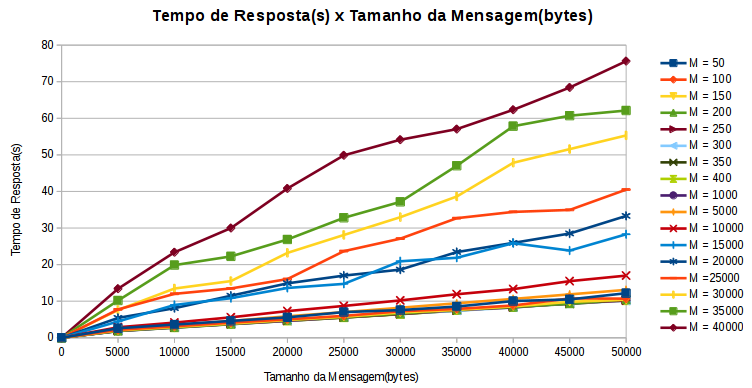
\includegraphics[scale=0.7]{figuras/A.png}
\caption{Gráfico do Tempo de Resposta x Tamanho da Mensagem para o Cenário A}
\label{fig:tempo_respostaXtamanho_msg_A}
\end{figure}

%%%%%%%%%%%%

Através dos testes, percebeu-se que o melhor resultado obtido foi com M igual a 300. Foi feita uma comparação de desempenho entre o primeiro trabalho(rodando na mesma configuração de cenário) e o segundo trabalho com M igual a 300. O resultado está ilustrado na Figura \ref{fig:tempo_respostaXtamanho_msg_A_T1}.

No primeiro trabalho, o intervalo de índices que cada escravo deve executar é calculada através da divisão do tamanho total dos índices pelo número de escravos registrados, no caso dessa configuração existem 12 escravos. 

A primeira coisa a se notar é que o desempenho do segundo trabalho, com M igual a 300, é muito melhor do que o primeiro, chegando a ser aproximadamente 4 vezes mais rápido. Isso pode ser explicado, para o trabalho 2, pelo fato de que para esse valor de M são gerados vários pequenos trabalhos, aumentando o nível de paralelismo, e, assim, permitindo uma melhora no tempo de resposta. Já para o primeiro trabalho são produzidos exatamente 12 trabalhos, fazendo com que cada escravo tenha que processar 6670 índices aproximadamente.

\begin{figure}[!htb]
\centering
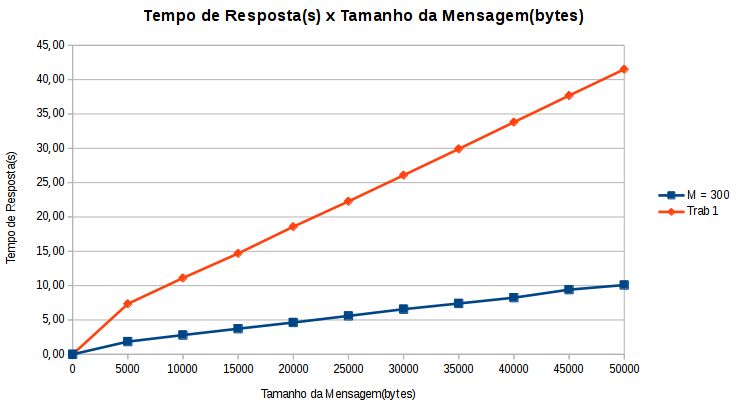
\includegraphics[scale=0.7]{figuras/A_T1.png}
\caption{Gráfico do Tempo de Resposta x Tamanho da Mensagem comparando o melhor M com o 1º trabalho - Cenário A}
\label{fig:tempo_respostaXtamanho_msg_A_T1}
\end{figure}

\section{Cenário B}
O cenário B, também consistia em 3 máquinas distintas, porém duas máquinas executavam 4 aplicações de escravo e uma executava 8, totalizando 16 escravos. A aplicação do mestre e do cliente também foram executadas em uma outra máquina. No dia dos testes do cenário B havia quatro grupos realizando testes, e, dessa forma, ocorreram algumas perturbações nos gráficos, porém elas não atrapalharam a realização das análises de desempenho.

A Figura \ref{fig:tempo_respostaXtamanho_msg_B} apresenta o gráfico dos resultados obtidos para o cenário B com vários valores de M.

Observando o gráfico, percebe-se que da mesma forma que ocorreu para o cenário A, à medida que o parâmetro M aumenta, o tempo de resposta também aumenta. Apesar de terem ocorridos algumas perturbações durante os testes, nota-se que o desempenho do segundo trabalho no cenário B é muito próximo do obtido no cenário A, mesmo com um computador sobrecarregado com 8 escravos. 

Isso já era esperado, visto que, nessa segunda implementação o escravo era capaz de realizar o controle de consumo dos trabalhos, já que um novo trabalho só era obtido quando o atual tivesse terminado. Assim, no computador que está muito sobrecarregado, a execução do trabalho irá demorar, porém, da mesma forma, a obtenção de um novo trabalho irá demorar, fazendo com que outros escravos que estejam disponíveis possam pegar o restante dos trabalho. Dessa forma, não ocorre perda significativa no desempenho.

Nota-se que para valores de M grandes, acima de 5000, o tempo de resposta aumentou quando comparado ao cenário A, e, também, pode se perceber oscilações para esses valores. Isso pode ter ocorrido pelo fato de que haviam 4 grupos realizando os testes no laboratório, e, como os testes eram executados na mesma rede, para mensagens maiores, o \textit{overhead} de comunicação acabou aumentando.

Os melhores resultados para os tempos de resposta foram obtidos com M de 1000 para baixo, sendo que para esses valores os resultados foram muito próximos. Da mesma forma que ocorreu para o cenário A, não foi possível observar com clareza os tempos de resposta obtidos para esses pequenos valores, por ficarem sobrepostos no gráfico. Porém, pelos testes realizados os melhores resultados foram obtidos com M igual a 400.

\begin{figure}[!htb]
\centering
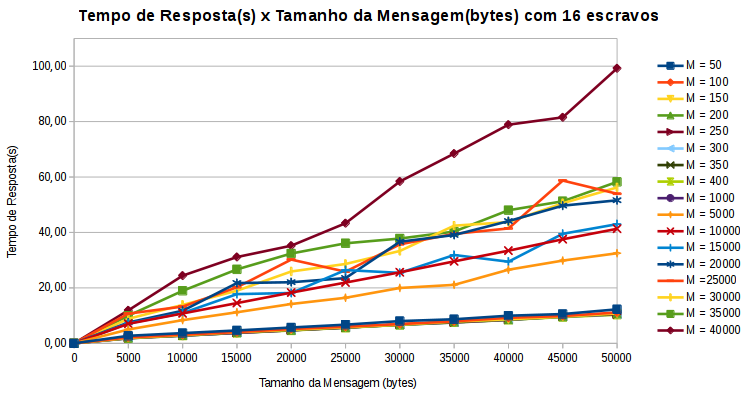
\includegraphics[scale=0.7]{figuras/B.png}
\caption{Gráfico do Tempo de Resposta x Tamanho da Mensagem para o Cenário B}
\label{fig:tempo_respostaXtamanho_msg_B}
\end{figure}

Também foi realizada uma comparação com a implementação do 1º trabalho na configuração do cenário B, o resultado está ilustrado na Figura \ref{fig:tempo_respostaXtamanho_msg_B_T1}.

É possível observar que o tempo de resposta da implementação do 2º trabalho é menor do que o 1º. Isso já era esperado visto que, existe uma máquina sobrecarregada executando 8 escravos. Na primeira implementação a divisão é feita igualmente entre todos os escravos, com isso, a máquina que possui 8 escravos recebe mais trabalhos do que as outras duas, nesse caso o dobro. Isso faz com que a máquina sobrecarregada demore ainda mais para executar os trabalhos, aumentando, assim, o tempo de resposta. 
Já no segundo trabalho esse problema não ocorre devido ao controle de consumo que o escravo é capaz de realizar.

\begin{figure}[!htb]
\centering
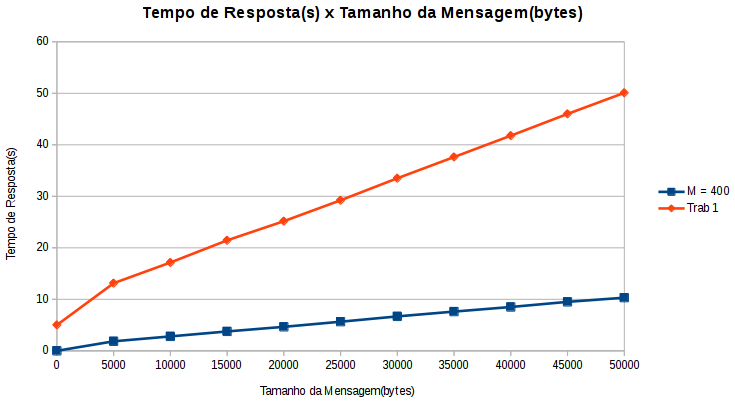
\includegraphics[scale=0.7]{figuras/B_T1.png}
\caption{Gráfico do Tempo de Resposta x Tamanho da Mensagem comparando o melhor M com o 1º trabalho - Cenário B}
\label{fig:tempo_respostaXtamanho_msg_B_T1}
\end{figure}


\section{Comparação entre Cenários}

A Figura \ref{fig:tempo_respostaXtamanho_msg_T2_AxB} apresenta uma comparação dos tempos de resposta obtidos para o segundo trabalho utilizando os dois cenários de testes e escolhendo-se o melhor M. Para o cenário A foi utilizado M igual a 300 e para o cenário B foi usado M igual a 400.

Como já foi dito na seção anterior. É possível perceber que os cenários A e B possuíram resultados semelhantes.
Mesmo com uma máquina sobrecarregada no cenário B, não houve um aumento do tempo de resposta. Isso já era esperado visto que nessa implementação ocorre o controle de consumo pelo escravo, dessa forma, a máquina mais sobrecarregada, executa menos trabalhos do que as outras, não compromentendo muito o tempo de resposta.

\begin{figure}[!htb]
\centering
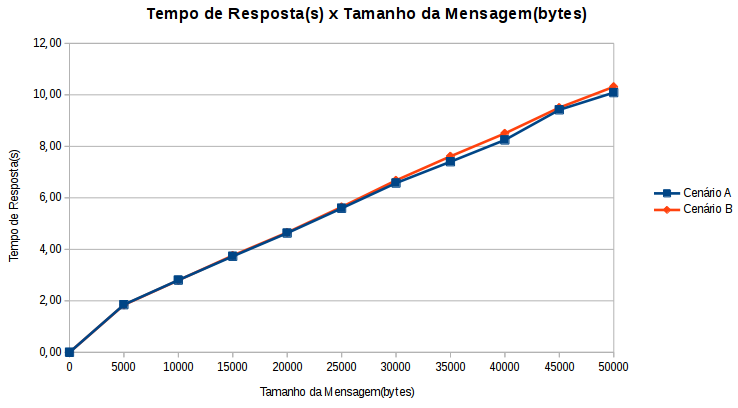
\includegraphics[scale=0.7]{figuras/T2_AxB.png}
\caption{Gráfico do Tempo de Resposta x Tamanho da Mensagem para o melhor M em Diferentes Cenários}
\label{fig:tempo_respostaXtamanho_msg_T2_AxB}
\end{figure}

A Figura \ref{fig:tempo_respostaXtamanho_msg_T1_AxB} apresenta uma comparação dos tempos de resposta obtidos para o primeiro trabalho utilizando os dois cenários de testes.

Nesse caso, já é possível perceber que no cenário B, onde existe uma sobrecarga em uma máquina, o tempo de resposta é maior do quando comparado ao cenário A. Como no primeiro trabalho não havia controle de consumo, a divisão era feita de forma igual entre os diversos escravos. Assim, a máquina sobrecarregada demorava para executar os trabalhos, fazendo com que o tempo de resposta aumentasse.

\begin{figure}[!htb]
\centering
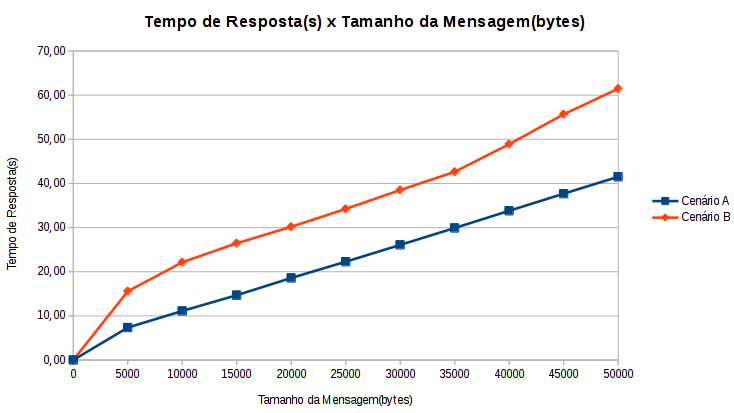
\includegraphics[scale=0.7]{figuras/T1_AxB.png}
\caption{Gráfico do Tempo de Resposta x Tamanho da Mensagem para o 1º trabalho em Diferentes Cenários}
\label{fig:tempo_respostaXtamanho_msg_T1_AxB}
\end{figure}


% Conclusão
% ---
\chapter{Conclusão}

Ao final do trabalho, foi possível perceber as vantagens de se utilizar troca de mensagens em uma aplicação distribuída. 

Os resultados obtidos mostraram que mesmo em um cenário onde uma máquina está sobrecarregada o tempo de resposta não é muito afetado devido ao controle de fluxo proporcionado por esse tipo de implementação. Diferentemente, no primeiro trabalho, isso não ocorre, e assim, em um cenário onde há uma sobrecarga em uma máquina, o tempo de resposta é afetado consideravelmente.

Algumas vantagens puderam ser notadas nesse segundo trabalho ao se utilizar troca de mensagens. A primeira é o desacoplamento espacial obtido, onde as entidades, nesse caso mestre e escravo, não precisavam conhecer umas as outras.

Outra vantagem é o desacoplamento temporal, que permite ao escravos poderem chegar e sair sem alterar o funcionamento do sistema. Isso fez com que a interface de \textit{SlaveManager} pudesse ser completamente removida, visto que, o gerenciamento de escravos não era mais necessário. 

Outro ponto interessante que pode se destacar é a simplicidade de implementação do mestre para esse segundo trabalho, quando comparado ao primeiro. Devido ao desacoplamento temporal e espacial, todos os serviços relacionados ao gerenciamento dos escravos e os serviços de \textit{rebind} e checkpoint puderam ser removidos.

Apesar das vantagens citadas, existe um ponto negativo que pode ser notado ao se utilizar esse tipo de solução. Como a comunicação realizada de forma indireta, o mestre não possui informação nenhuma sobre a existência ou não de escravos. Dessa forma, caso ele receba uma requisição de um cliente, a única coisa que ele irá fazer é criar os subataques e esperar, até que todos estejam terminados para enviar uma resposta ao cliente. No primeiro trabalho, o mestre possuía uma lista com os escravos ativos, e caso, ele recebesse uma solicitação de ataque ele poderia verificar se essa lista estava vazia ou não, caso estivesse, poderia traçar alguma estratégia para finalizar o ataque, seja lançando uma exceção para o cliente ou realizando por si mesmo o ataque.




% ----------------------------------------------------------
% ELEMENTOS PÓS-TEXTUAIS
% ----------------------------------------------------------
\postextual


% ----------------------------------------------------------
% Referências bibliográficas
% ----------------------------------------------------------
%\bibliography{referencias} %% REFERENCIA AO ARQUIVO .bib

\end{document}
\grid
